%!TEX options = -shell-escape

\documentclass[12pt]{report}
\usepackage[a4paper,twoside,top=20mm,bottom=20mm,inner=30mm,outer=25mm]{geometry}
\usepackage[utf8]{inputenc}
\usepackage[greek,english]{babel}
\usepackage[scaled=0.86]{couriers}
\usepackage[toc,page,title,titletoc]{appendix}
\usepackage[pdfpagelabels,unicode]{hyperref}
\usepackage{bookmark}
\usepackage[fixlanguage]{babelbib}
\selectbiblanguage{greek}
\usepackage{titlesec}
\usepackage{etoolbox}
\usepackage{graphicx}
\usepackage{array}
\usepackage{amsmath}
\usepackage{minted}
\usepackage{subcaption}
\captionsetup{compatibility=false}
\graphicspath{ {images/} }
\usepackage[noend]{algpseudocode}
\usepackage{algorithm}
\usepackage{afterpage}
\usepackage{comment}
\usepackage{float}

\newcommand\blankpage{%
    \null
    \thispagestyle{empty}%
    \addtocounter{page}{-1}%
    \newpage}

\hypersetup{
  colorlinks=true,
  % linkcolor=green,
  citecolor=red,
  % filecolor=blue,
  urlcolor=blue,
  % pdftitle=,
  % pdfauthor=,
  % pdfsubject=,
  % pdfkeywords=
}

\setcounter{secnumdepth}{3}
\setcounter{tocdepth}{3}

\titleformat{\chapter}
  {\normalfont\LARGE\bfseries}{\thechapter}{1em}{}
\titlespacing*{\chapter}{0pt}{3.5ex plus 1ex minus .2ex}{2.3ex plus .2ex}

\makeatletter
\patchcmd\@resets@pp{%
  \def\Hy@chapapp{\appendixname }%
}{%
  \def\Hy@chapapp{appendix}%
}{}{\errmessage{Cannot patch \string\@resets@pp}}
\patchcmd\@resets@ppsub{%
  \def\Hy@chapapp{\appendixname }%
}{%
  \def\Hy@chapapp{appendix}%
}{}{\errmessage{Cannot patch \string\@resets@pp}}
\makeatother

\addto{\captionsgreek}{\renewcommand{\appendixpagename}{Παραρτήματα}}
\addto{\captionsgreek}{\renewcommand{\appendixtocname}{Παραρτήματα}}
\addto{\captionsgreek}{\renewcommand{\appendixname}{Παράρτημα}}

\begin{document}
\selectlanguage{greek}

\hypersetup{pageanchor=false}

\begin{titlepage}
  \centering
  
\includegraphics[width=0.15\textwidth]{pyrforos}\par\vspace{1cm}
  {\scshape\LARGE Εθνικό Μετσόβιο Πολυτεχνείο\\
  Σχολή Ηλεκτρολόγων Μηχανικών και Μηχανικών Η/Υ\par}
  \vspace{1cm}
  {\scshape\Large Εργασία στο Μεταπτυχιακό Μάθημα\\
  Διαχείριση Τεχνολογιών στο Ηλεκτρονικό Εμπόριο\par}
  \vspace{1.5cm}
  {\Large\bfseries Ανάπτυξη Ιστοσελίδας Ηλεκτρονικών Δημοπρασιών\par}
  \vspace{2cm}
  {\large Δημήτριος Πολίτης (ΥΔ)\par}
  \vfill
  Επιβλέπων \par
  Καθ. Ευστάθιος Συκάς

  \vfill

% Bottom of the page
  {\large \today\par}
  \afterpage{\blankpage}
\end{titlepage}

\tableofcontents
\thispagestyle{empty}

\listoffigures
\thispagestyle{empty}

\begin{abstract}
Στο παρόν παρουσιάζεται η λειτουργία και η διαδικασία ανάπτυξης μιας ιστοσελίδας δημοπρασιών. Αρχικά  γίνεται αναφορά στις βασικές έννοιες του ηλεκτρονικού εμπορίου και στη συνέχεια περιγράφεται αναλυτικά η διαδικασία δημιουργίας ενός ιστοτόπου ηλεκτρονικών δημοπρασιών με τη χρήση αυτοματοποιημένων εργαλείων (\textlatin{phpProBid, vagrant}). Η εργασία είναι διαθέσιμη από το σύνδεσμο \textlatin{\url{https://github.com/dpolitis/e-commerce}}.

\vspace{10mm}

\noindent \textbf{Λέξεις κλειδιά:} Ηλεκτρονικό Εμπόριο, Ηλεκτρονική Δημοπρασία, Ανοιχτός Κώδικας, Εξυπηρετητής Ιστοσελίδων, Διαδίκτυο.
\end{abstract}

\hypersetup{pageanchor=true}
\clearpage
\pagenumbering{arabic}

\chapter{Εισαγωγή}\label{ch1}
\section{Εισαγωγή}
Η εποχή του διαδικτύου επιβάλει την αναθεώρηση των παραδοσιακών τρόπων διεξαγωγής του εμπορίου, μέσω φυσικής επαφής. Πλέον μεγάλο ποσοστό των εμπορικών συναλλαγών, τόσο μεταξύ επιχειρήσεων, όσο και μεταξύ ιδιωτών και επιχειρήσεων, πραγματοποιούνται με ηλεκτρονικά μέσα.

Η δημιουργία, η συντήρηση και η ανανέωση του περιεχομένου των ιστοτόπων ηλεκτρονικών αγορών αποτελεί μοχλό μεγέθυνσης των πωλήσεων και σε βάθος χρόνου, του κύκλου εργασιών.

\section{Ηλεκτρονικό Εμπόριο}
\subsection{Ορισμοί - Έννοιες}
Το Ηλεκτρονικό Εμπόριο (ΗΕ) περιγράφει τη διαδικασία αγοράς, πώλησης, μεταφοράς ή ανταλλαγής προϊόντων, υπηρεσιών ή/και πληροφοριών μέσω δικτύων υπολογιστών, περιλαμβανομένου και του Διαδικτύου~\cite{turban_outland_king_lee_liang_turban_2018}. Το ΗΕ μπορεί να οριστεί από τις παρακάτω σκοπιές:
  \paragraph{Επιχειρησιακή Διεργασία.} Από την σκοπιά των επιχειρησιακών διεργασιών το ΗΕ αφορά στην εκτέλεση των διεργασιών με ηλεκτρονικό τρόπο, ολοκληρώνοντας ηλεκτρονικές διεργασίες μέσω δικτύων Η/Υ.
  \paragraph{Εξυπηρέτηση.} Από τη σκοπιά των επιχειρήσεων, το ΗΕ είναι ένα εργαλείο που απευθύνεται στη επιθυμία των κυβερνήσεων, των εταιριών, των πελατών και της διοίκησης να περικόψουν το κόστος των υπηρεσιών ενώ ταυτόχρονα να βελτιώσουν την παρεχόμενη ποιότητα των υπηρεσιών και ταχύτητα εξυπηρέτησης.
  \paragraph{Εκπαίδευση.} Από τη σκοπιά της εκπαίδευσης, το ΗΕ παρέχει την δυνατότητα εκπαίδευσης και επιμόρφωσης \textlatin{online} σε σχολεία, πανεπιστήμια και επιχειρήσεις.
  \paragraph{Συνεργατική.} Από τη σκοπιά της συνεργασίας είναι το πλαίσιο της ενδοεπιχειρησιακής και διαεπιχειρησιακής συνέχειας.
  \paragraph{Κοινωνική.} Από την κοινωνική σκοπιά, το ΗΕ παρέχει μια θέση συγκέντρωσης μελών της κοινωνίας για εκμάθηση, συνδιαλλαγή και συνεργασία.

Πολλές φορές το ΗΕ συγχέεται με το Ηλεκτρονικό Επιχειρείν, μια πιο ευρεία έννοια. Το Ηλεκτρονικό Επιχειρείν αναφέρεται στον ευρύτερο ορισμό του ΗΕ, όχι μόνο στην αγορά και την πώληση των αγαθών αλλά και επίσης στην εξυπηρέτηση πελατών, στη συνεργασία με επιχειρηματικούς εταίρους, στη διεξαγωγή ηλεκτρονικής εκπαίδευσης και την διεξαγωγή ηλεκτρονικών συναλλαγών εντός των ορίων του οργανισμού.

Σύμφωνα με το~\cite{chen_2005} το Ηλεκτρονικό Επιχειρείν είναι η χρήση του Διαδικτύου και άλλων τεχνολογιών της πληροφορικής για την υποστήριξη του εμπορίου και τη βελτίωση της απόδοσης μιας επιχείρησης.

\subsection{Αμιγές και Μερικό ΗΕ}
Το ηλεκτρονικό εμπόριο μπορεί να πάρει πολλές μορφές ανάλογα με το βαθμό ψηφιοποίησης των παρακάτω παραγόντων:
\begin{itemize}
  \item του προϊόντος - υπηρεσίας προς πώληση
  \item της διαδικασίας (για παράδειγμα παραγγελία ή πληρωμή)
  \item της μεθόδου διανομής
\end{itemize}

Στο~\cite{choi_stahl_whinston_1997} παρουσιάζεται ένα μοντέλο που περιγράφει τους πιθανούς συνδυασμούς αυτών των τριών διαστάσεων. Ένα προϊόν μπορεί να είναι φυσικό ή ψηφιακό, η μέθοδος διανομής μπορεί να είναι φυσική η ηλεκτρονική, Η διαδικασία μπορεί αναλόγως να είναι φυσική η ψηφιακή. Αυτές οι εναλλακτικές καταστασεις δημιουργούν οκτώ τρισδιάστατους κύβους. Στο παραδοσιακό εμπόριο όλες οι διαστάσεις είναι φυσικές, ενώ στο αμιγές ΗΕ όλες οι διαστάσεις είναι ψηφιακές. Όλοι οι άλλοι κύβοι περιλαμβάνουν ένα μείγμα ψηφιακών και φυσικών διαστάσεων. Η περιγραφή αυτή γίνεται κατανοητή εφόσον παρατηρήσουμε το σχήμα~\ref{fig:ec_dimensions}.
\begin{figure}[h]
\centering
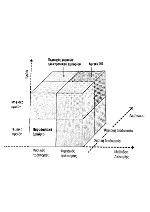
\includegraphics[width=0.8\textwidth, height=8cm]{ec-dimensions}
\caption{Διάγραμμα τύπων ΗΕ}
\label{fig:ec_dimensions}
\end{figure}
Εάν υπάρχει έστω και μια ψηφιακή διάσταση, τότε έχουμε μερικό ΗΕ. Αναλόγως με τον τρόπο τον οποίο διεξάγουν την πώληση και τη διανομή ενός εμπορεύματος, οι οργανισμοί - εταιρίες μπορούν να κατηγοριοποιηθούν όπως παρακάτω:
\begin{itemize}
  \item Παραδοσιακοί Οργανισμοί (παλαιάς οικονομίας).
  \item Εικονικοί ή ηλεκτρονικοί οργανισμοί.
  \item Οργανισμοί μερικού ΗΕ.
\end{itemize}
Οι αμιγώς φυσικοί οργανισμοί αναφέρονται ως παραδοσιακοί οργανισμοί, ενώ εταιρίες οι οποίες χρησιμοποιούν μόνο ΗΕ θεωρούνται εικονικοί οργανισμοί. Οι οργανισμοί μερικού ΗΕ είναι εκείνοι οι οργανισμοί που επιτελούν μερικές δραστηριότητες ηλεκτρονικού εμπορίου, ενώ οι κύρια δραστηριότητά τους πραγματοποιείται με φυσικό τρόπο.

\subsection{Τύποι Ηλεκτρονικού Εμπορίου}
Μια συνηθισμένη κατάταξη του ΗΕ είναι με βάση την φύση της συνναλλαγής ή με τη σχέση ανάμεσα στους συμμετέχοντες, όπως παρακάτω:
\begin{itemize}
  \item \textlatin{Bussiness to Bussiness (B2B)}, Όλοι οι συμμετέχοντες είναι επιχειρήσεις ή άλλοι οργανισμοί.
  \item \textlatin{Bussiness to Consumer (B2C)}, Περιλαμβάνει συναλλαγές λιανικού εμπορίου προϊόντων ή υπηρεσιών από επιχειρήσεις προς μεμονομένους αγοραστές.
  \item \textlatin{Bussiness to Government (B2G)}, Περιλαμβάνει συναλλαγές παροχής υπηρεσιών ή αγαθών από επιχειρήσεις προς το δημόσιο τομέα.
  \item \textlatin{Government to Bussiness (G2B)}, Περιλαμβάνει συναλλαγές παροχής υπηρεσιών από το κράτος προς τον ιδιωτικό τομέα.
  \item \textlatin{Consumer to Consumer (C2C)}, Περιλαμβάνει συναλλαγές λιανικού εμπορίου προϊόντων ή υπηρεσιών από ιδιώτες προς ιδιώτες.
  \item \textlatin{Government to Consumer (G2C)}, Περιλαμβάνει συναλλαγές παροχής υπηρεσιών από το κράτος προς τον ιδιώτες.
\end{itemize}

\section{Ηλεκτρονικές Θέσεις Αγορών}
Σύμφωνα με τον~\cite{bakos_1998}, οι αγορές διαδραματίζουν ουσιώδη ρόλο στην οικονομία διευκολύνοντας την ανταλλαγή πληροφοριών, αγαθών, υπηρεσιών και πληρωμών. Οι αγορές (ηλεκτρονικές ή όχι) έχουν τρεις κύριες λειτουργίες:
\begin{itemize}
  \item Ταίριασμα αγοραστών - πωλητών.
  \item Παροχή ενός θεσμικού πλαισίου (νομικού - ρυθμιστικού) για την αποτελεσματική λειτουργία τους.
  \item Διευκόλυνση ανταλλαγή πληροφοριών, αγαθών κτλ, όπως αναφέρθηκε παραπάνω.
\end{itemize}

\subsection{Ηλεκτρονικές Θέσεις Αγορών}
Η βασική θέση για τη διεξαγωγή συναλλαγών ΗΕ είναι η ηλεκτρονική αγορά. Μια Ηλεκτρονική θέση Αγορών είναι μια εικονική θέση αγορών, στην οποία συναντώνται και διεξάγουν διάφορους τύπους συναλλαγών πωλητές και αγοραστές. Η λειτουργίες μιας ηλεκτρονικής θέσης αγορών είναι πανομοιότυπες με αυτές μιας φυσικής αγοράς. Τα ηλεκτρονικά μέσα όμως κάνουν τις αγορές περισσότερο αποδοτικές, παρέχοντας πλήθος ενημερωμένων πληροφοριών σε όλους τους εμπλεκομένους. Διακρίνονται σε:
\begin{itemize}
  \item Ιδιωτικές: Η θέση αγορών ανήκει σε ένα μόνο φορέα - εταιρία, η οποία τη διαχειρίζεται και είτε πωλεί τα δικά της προϊόντα (ένας προς πολλούς), είτε προσκαλεί προμηθευτές (πολλοί προς έναν).
  \item Δημόσιες: Ανήκουν σε κάποιο τρίτο και περιλαμβάνουν πολλούς αγοραστές και πωλητές.
  \item Θέσεις αγορών με πράκτορες: Οι πράκτορες λογισμικού συγκεντρώνουν πληροφορίες σχετικά με προϊόντα και τιμές και τα παρουσιάζουν σε πιθανούς αγοραστές ή πωλητές. Στην πιο εξελιγμένη τους μορφή οι πράκτορες αγοραστή και πωλητή μπορούν να αλληλεπιδρούν σε μια πλήρως αυτοματοποιημένη αγορά~\cite{turban_outland_king_lee_liang_turban_2018}.
\end{itemize}

\subsection{Οι Δημοπρασίες ως Μηχανισμοί Αγορών ΗΕ}
Ένας από τους πιο ενδιαφέροντες μηχανισμούς της αγοράς στο ηλεκτρονικό εμπόριο είναι οι ηλεκτρονικές δημοπρασίες. Αυτές Χρησιμοποιούνται στα \textlatin{B2C, B2B, C2C, G2B, G2C} κ.α. Μια δημοπρασία είναι ένας μηχανισμός αγοράς, που χρησιμοποιεί μια ανταγωνιστική διαδικασία κατά την οποία, ένας πωλητής δέχεται ακολουθιακές προσφορές από αγοραστές (προωθητική δημοπρασία) ή ένας αγοραστής δέχεται προσφορές από πωλητές (αντίστροφη δημοπρασία). Είναι δυνατό να λάβουν χώρα:
\begin{itemize}
  \item Σε δημόσιες τοποθεσίες δημοπρασιών, όπως το \textlatin{EBay}.
  \item Κατόπιν προσκλήσης σε ιδιωτικές δημοπρασίες.
\end{itemize}

Το παρόν πραγματεύεται την ανάπτυξη μιας ιστοσελίδας ηλεκτρονικών δημοπρασιών πλήρους λειτουργικότητας. Στα επόμενα παρουσιάζεται η διαδικασία ανάπτυξης, τα εργαλεία που χρησιμοποιήθηκαν και γίνεται μια συνοπτική αναφορά στις λειτουργίες που παρέχει η υπόψη ιστοσελίδα ηλεκτρονικών δημοπρασιών.

\chapter{Ανάπτυξη Ιστοσελίδας Ηλεκτρονικών Δημοπρασιών}\label{ch2}
Για την ανάπτυξη της ιστοσελίδας της εργασίας χρησιμοποιήθηκε πλήθος εργαλείων, τα οποία στην πλειονότητά τους βρίσκονται διαθέσιμα δωρεάν στο Διαδίκτυο (\textlatin{Open Source Software}). Στα επόμενα γίνεται μια σύντομη αναφορά στα εργαλεία που χρησιμοποιήθηκαν και στη διαδικασία της ανάπτυξης.

\section{\textlatin{\textlatin{Vagrant (Open Source VM Provissioner)}}}\label{vagrant}
Το \textlatin{Vagrant} είναι ένα εργαλείο δημιουργίας και διαχείρησης εικονικών μηχανών με τη χρήση μιας εξαιρετικά απλοποιημένης διαδικασίας~\cite{vagrant_by_hashicorp}. Το εργαλείο αυτό δίνει έμφαση στην αυτοματοποιημένη διαχείριση των εικονικών μηχανών και μειώνει σημαντικά το χρόνο δημιουργίας και παραμετροποίησης ενός \textlatin{development server}.

Είναι γραμμένο στη γλώσσα προγραμματισμού \textlatin{Ruby} και αποτελεί έναν ενιαίο τρόπο επικοινωνίας με δίάφορους \textlatin{providers} εικονικών μηχανών (όπως \textlatin{VirtualBox, VMware, AWS} κ.α.). Με τον τρόπο αυτό είναι δυνατή η δημιουργία εικονικών μηχανών με τις επιθυμητές παραμέτρους στον μικρότερο δυνατό χρόνο. Παράλληλα, για την εγκατάσταση πακέτων λογισμικού αλλά και παραμετροποίηση σε επίπεδο λειτουργικού συστήματος (ΛΣ), είναι δυνατή η συνεργασία με ευρέως διαδεδομένα \textlatin{provisioning tools}, όπως \textlatin{Chef, Puppet, Ansible} ακόμα και με απλά \textlatin{shell scripts}.

Το μεγαλύτερο ίσως πλεονέκτημα του υπόψη εργαλείου είναι η δυνατότητα παροχής στους προγραμματιστές ενός ενιαίου περιβάλλοντος, το οποίο είναι σταθερό και όσο κοντά γίνεται στο παραγωγικό εξυπηρετητή. Επίσης επειδή η παραμετροποίηση γίνεται με αυτόματο τρόπο, αφαιρείται από τους προγραμματιστές το βάρος της δημιουργίας, συντήρησης και αποσφαλμάτωσης του περιβάλλοντος ανάπτυξης.

Η αρχή λειτουργίας του \textlatin{Vagrant} στηρίζεται στην ύπαρξη μιας εικονικής μηχανής στελέχους (\textlatin{template/vagrant box}), η οποία είναι διαθέσιμη από τα επίσημα αποθετήρια \textlatin{\url{https://vagrantcloud.com/boxes/search}} είτε μπορεί να είναι δική μας. Κατόπιν μέσω μιας διαδικασίας κλωνοποίησης και εφαρμογής παραμέτρων, εντελώς διαφανούς για το χρήστη, αποδίδεται η εικονική μηχανή.

Όλα τα παραπάνω γίνονται με την εκτέλεση της εντολής \textlatin{\texttt{vagrant}} ακολουθούμενης από το αντίστοιχο \textlatin{switch}. Για παράδειγμα, η παρακάτω ακολουθία εντολών κατεβάζει μια εικονική μηχανή \textlatin{ubuntu 64bit} από το επίσημο αποθετήριο και την θέτει σε λειτουργία με τη βοήθεια του \textlatin{VirtualBox}.
\selectlanguage{english}
\begin{Verbatim}
  $ vagrant box add ubuntu/xenial64
  $ vagrant init
  $ vagrant up --provider=virtualbox
\end{Verbatim}
\selectlanguage{greek}
Για τη φιλοξενία του ιστοτόπου της εργασίας χρησιμοποιήθηκε μια μηχανή \textlatin{centos7 64bit} από το επίσημο αποθετήριο. Επειδή η ανάπτυξη έγινε σε \textlatin{Fedora Linux}, χρησιμοποιήθηκε ως \textlatin{Virtualization provider} το παρεχόμενο από το ίδιο το λειτουργικό \textlatin{KVM / libvirt}. Στην συνέχεια με τη χρήση \textlatin{shell provissioner} έγινε η εγκατάσταση και παραμετροποίηση της βάσης δεδομένων (\textlatin{mariadb}) και του \textlatin{webserver (apache 2.4, php 5.4)}. Με τη χρήση του ίδιου \textlatin{provissioner} συγχρονίστηκε ο κώδικας και τέθηκαν τα σωστά \textlatin{filesystem permissions}.

Όλα τα παραπάνω ορίζονται στο αρχείο \textlatin{\texttt{Vagrantfile}} το οποίο παρατίθεται στο Παράρτημα~\ref{AppA}.

\section{\textlatin{PHP ProBid (Propietary Auctions Engine)}}\label{phpprobid}
Το \textlatin{PHP ProBid} είναι μια μηχανή διαχείρησης διαδικασίας δημοπρασιών, η οποία λειτουργεί με τη χρήση αρθρωμάτων (\textlatin{modules}) για την επαύξηση των λειτουργιών. Στη βασική της έκδοση παρέχει την προγραμματιστική διεπαφή \textlatin{API} για τη σύνδεση με \textlatin{frontend} σε \textlatin{php}, με βασική μόνο λειτουργικότητα διεξαγωγής δημοπρασιών.

Στη συνέχεια με την προσθήκη \textlatin{modules} είναι δυνατή η διασύνδεση με το τραπεζικό σύστημα για τη διεξαγωγή πληρωμών μέσω \textlatin{paypal} ή τραπεζικών καρτών. Ενδεικτικά το συγκεκριμένο \textlatin{module} κοστίζει περίπου 80 Ευρώ.

Το \textlatin{PHP ProBid} στις τελευταίες του εκδόσεις έχει επεκταθεί από μια μηχανή διεξαγωγής δημοπρασιών σε ολοκληρωμένο σύστημα το οποίο μπορεί να υποστηρίξει ένα ηλεκτρονικό κατάστημα σε όλο το φάσμα των λειτουργιών του, από τη διαχείριση χρηστών, αποθεμάτων, καλαθιού αγορών, ενσωμάτωση πληρωμών, έκδοση τιμολογίων έως και την διαδικασία αποστολής στον τελικό αποδέκτη. Φυσικά όσο αυξάνεται η λειτουργικότητα, τόσο αυξάνεται και το κόστος αγοράς του λογισμικού.

Λόγω του ότι το \textlatin{PHP ProBid} είναι εμπορικό λογισμικό κλειστού κώδικα, ενσωματώνει τεχνικές κρυπτογράφησης του \textlatin{php} κώδικά του και απαιτεί μια \textlatin{on-line} βιβλιοθήκη αποκρυπτογράφησης. Αυτή παρέχεται ανεξάρτητα ως το \textlatin{Apache module IonCube~\url{https://ioncube.com}}. Στην ίδια ιστοσελίδα παρέχονται οδηγίες εγκατάστασης και ενεργοποίησής της βιβλιοθηκης.

Για τις ανάγκες τις εργασίας ενσωματώθηκε μόνο η βασική λειτουργικότητα, καθώς η ενσωμάτωση λειτουργιών πληρωμών κ.τ.λ. απαιτεί την αγορά των αντίστοιχων \textlatin{modules}.

\section{Διαδικασία Ανάπτυξης}
Μετά την εγκατάσταση της εικονικής μηχανής και του \textlatin{auctions engine} με τη χρήση του \textlatin{Vagrantfile}, όπως περιγράφηκε στο~\ref{vagrant}, ακολουθήθηκε η διαδικασία ανάπτυξης του \textlatin{frontend} και της διασύνδεσης με το \textlatin{PHP-ProBid API} σε γλώσσα \textlatin{php}.

Οι γραμμές 61-71 του \textlatin{Vagrantfile} του Παραρτήματος~\ref{AppA} φροντίζουν ώστε οι αλλαγές στον κώδικα που γίνονται τοπικά στον Η/Υ να συγχρονίζουν αυτόματα στην εικονική μηχανή, ώστε να είναι άμεσα εμφανείς στο \textlatin{web browser}.

Αρχικά υλοποιήθηκε το \textlatin{admin panel} με τι σελίδες διαχείρησης χρηστών και δικαιωμάτων. Στη συνέχεια υλοποιήθηκαν οι σελίδες \textlatin{login} για τους απλούς χρήστες και το \textlatin{admin panel}, ώστε να είναι έτοιμες για τα σενάρια αποσφαλμάτωσης. Έπειτα δημιουργήθηκε το αρχείο με τα μηνύματα της διεπαφής στα ελληνικά και τα αγγλικά, το οποίο εμπλουτίστηκε στη συνέχεια με νέο περιεχόμενο, κατά τη διαδικασία της ανάπτυξης.

Στα επόμενα στάδια δημιουργήθηκε η διεπαφή δημιουργίας μιας δημοπρασίας, με δυνατότητα ανάρτησης κειμένου, φωτογραφιών και άλλων πολυμέσων περιγραφής του προς πώληση προϊόντος. Τελευταία δημιουργήθηκε η διεπαφή πονταρίσματος (\textlatin{bidding}) με τις βασικές λειτουργίες αυτόματης ανανέωσης της σελίδας, λήξης της δημοπρασίας με χρονομέτρηση και ανάδειξη νικητή με βάση το ύψος της προσφοράς.

Με το πέρας της διαδικασίας ανάπτυξης δημιουργήθηκαν δοκιμαστικοί χρήστες και σενάρια δοκιμών για την αποσφαλμάτωση του κώδικα. Δοκιμάστηκαν πλήρη σενάρια και διορθώθηκαν σφάλματα, τα οποία είχαν να κάνουν με την μη σωστή αυτόματη ανανέωση του περιεχομένου της σελίδας.

\chapter{Περιγραφή της Ιστοσελίδας Ηλεκτρονικών Δημοπρασιών}\label{ch3}
Στο παρόν γίνεται σύντομη αναφορά στη λειτουργικότητα της ιστοσελίδας δημοπρασιών που αναπτύχθηκε όπως στο~\ref{ch2}. Παρατίθενται \textlatin{screenshots} με επεξηγήσεις για τις κύριες λειτουργίες της σελίδας.

\section{Λειτουργικότητα Ιστοσελίδας}
\subsection{\textlatin{Admin Panel}}
Το πρώτο πράγμα που βλέπει κάποιος όταν επισκέπτεται την ιστοσελίδα είναι η φόρμα εισόδου. Για τις ανάγκες της εφαρμογής έχουν δημιουργηθεί δυο διαφορετικές σελίδες εισόδου. Μια για το \textlatin{admin panel} και μια για το \textlatin{login} των λοιπών χρηστών. Στην εικόνα~\ref{fig:login_1} παρουσιάζεται η σελίδα εισόδου στο \textlatin{admin panel}.
\begin{figure}[H]
\centering
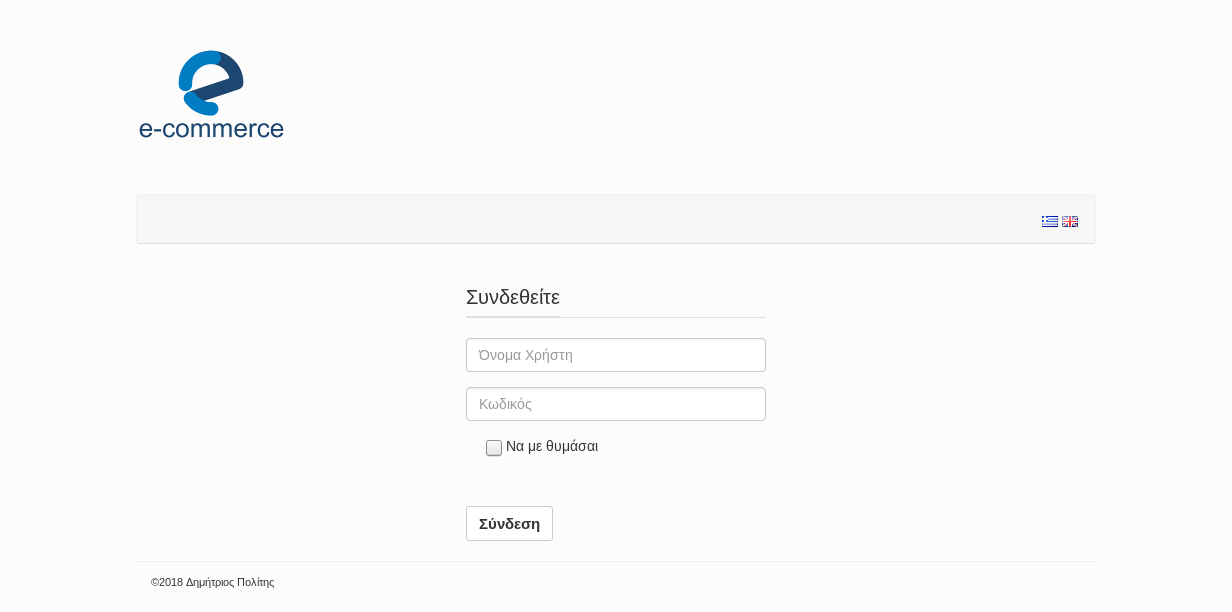
\includegraphics[width=0.8\textwidth, height=8cm]{Screenshot-2018-1-14-login-e-auctions}
\caption{Φόρμα Εισόδου \textlatin{Admin Panel}}
\label{fig:login_1}
\end{figure}

Παρόμοια είναι και η σελίδα εισόδου χρηστών, αλλά είναι προσβάσιμη μέσω διαφορετικού \textlatin{url}. Μετά την επιτυχή είσοδο στη σελίδα του \textlatin{admin panel} ο διαχειριστής μπαίνει στη σελίδα διαχείρησης χρηστών του ιστοτόπου. Από εδώ είναι δυνατή η δημιουργία, διαγραφή και τροποποίηση των χρηστών της πλατφόρμας. Επίσης, είναι δυνατή η ανάθεση ρόλων (πωλητή, αγοραστή, παρατηρητή ή διαχειριστή) και η αλλαγή συνθηματικών. Η φόρμα διαχείρησης χρηστών εμφανίζεται στην εικόνα~\ref{fig:user_admin}.
\begin{figure}[H]
\centering
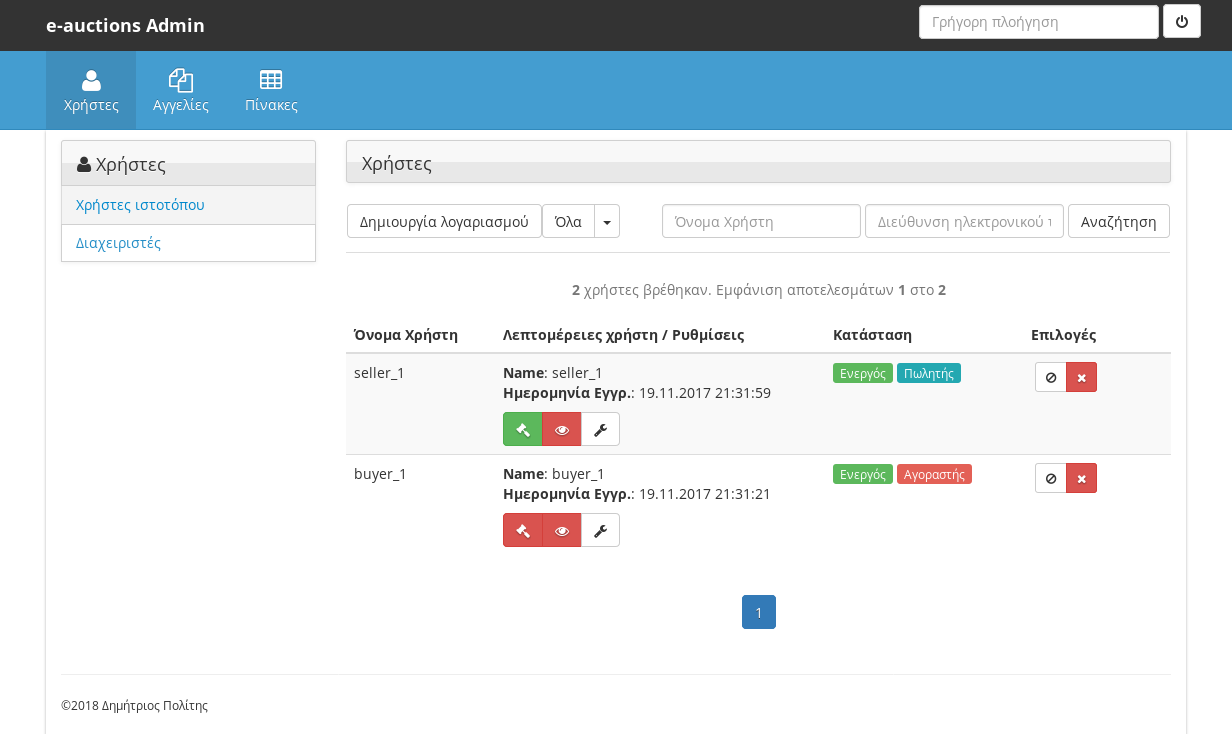
\includegraphics[width=0.8\textwidth, height=8cm]{Screenshot-2018-1-14-e-auctions-Admin-2}
\caption{Φόρμα Διαχείρησης Χρηστών}
\label{fig:user_admin}
\end{figure}

Στο επόμενο \textlatin{tab} εμφανίζονται τα εργαλεία της διαχείρισης όλων των δημοπρασιών (μόνο ακύρωση - διαγραφή, εικόνα~\ref{fig:auction_admin}).
\begin{figure}[H]
\centering
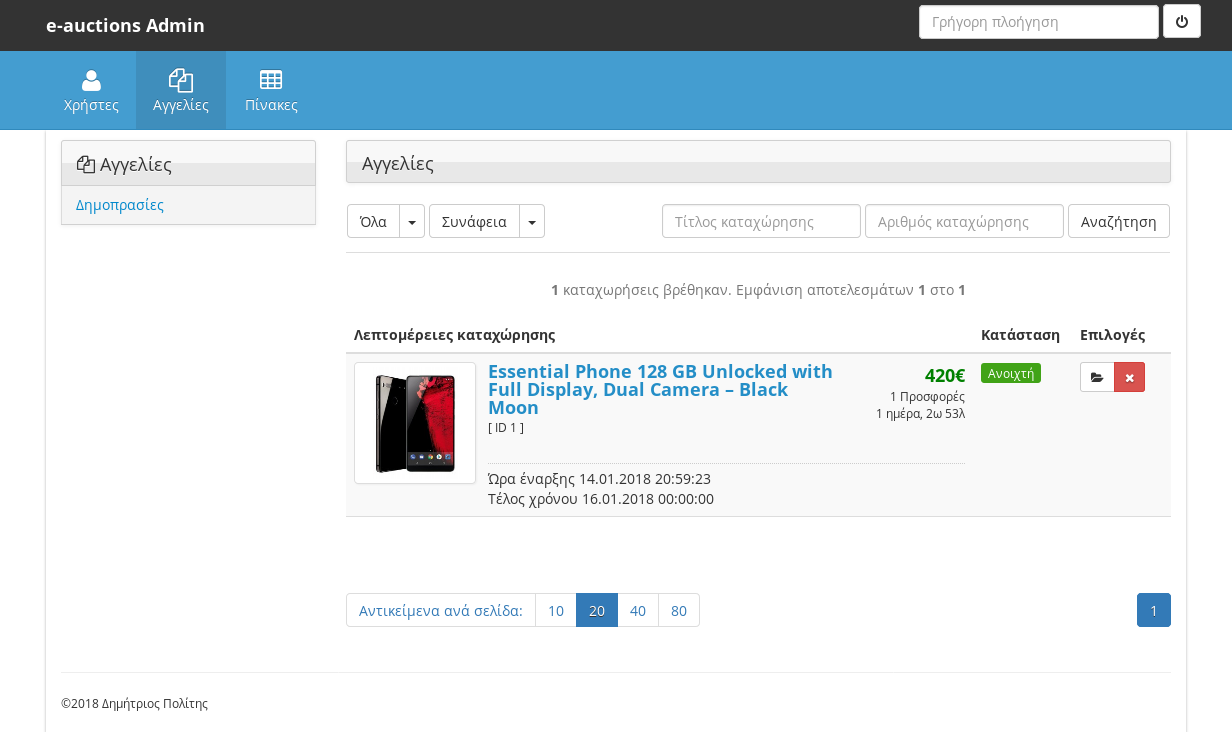
\includegraphics[width=0.8\textwidth, height=8cm]{Screenshot-2018-1-14-e-auctions-Admin-3}
\caption{Φόρμα Διαχείρησης Δημοπρασιών}
\label{fig:auction_admin}
\end{figure}

Το τελευταίο εργαλείο του \textlatin{admin panel} αφορά στη διαχείριση κατηγοριών προϊόντων. Εδώ καθορίζονται οι κατηγορίες στις οποίες καταχωρούνται τα προϊόντα κατά τη δημιουργία μιας δημοπρασίας. Είναι δυνατή η προσθήκη, διαγραφή και ενημέρωση της περιγραφής, του μοναδικού αναγνωριστικού και μιας προαιρετικής μικρογραφίας για την περιγραφή της κατηγορίας (εικόνα~\ref{fig:category_admin}).
\begin{figure}[H]
\centering
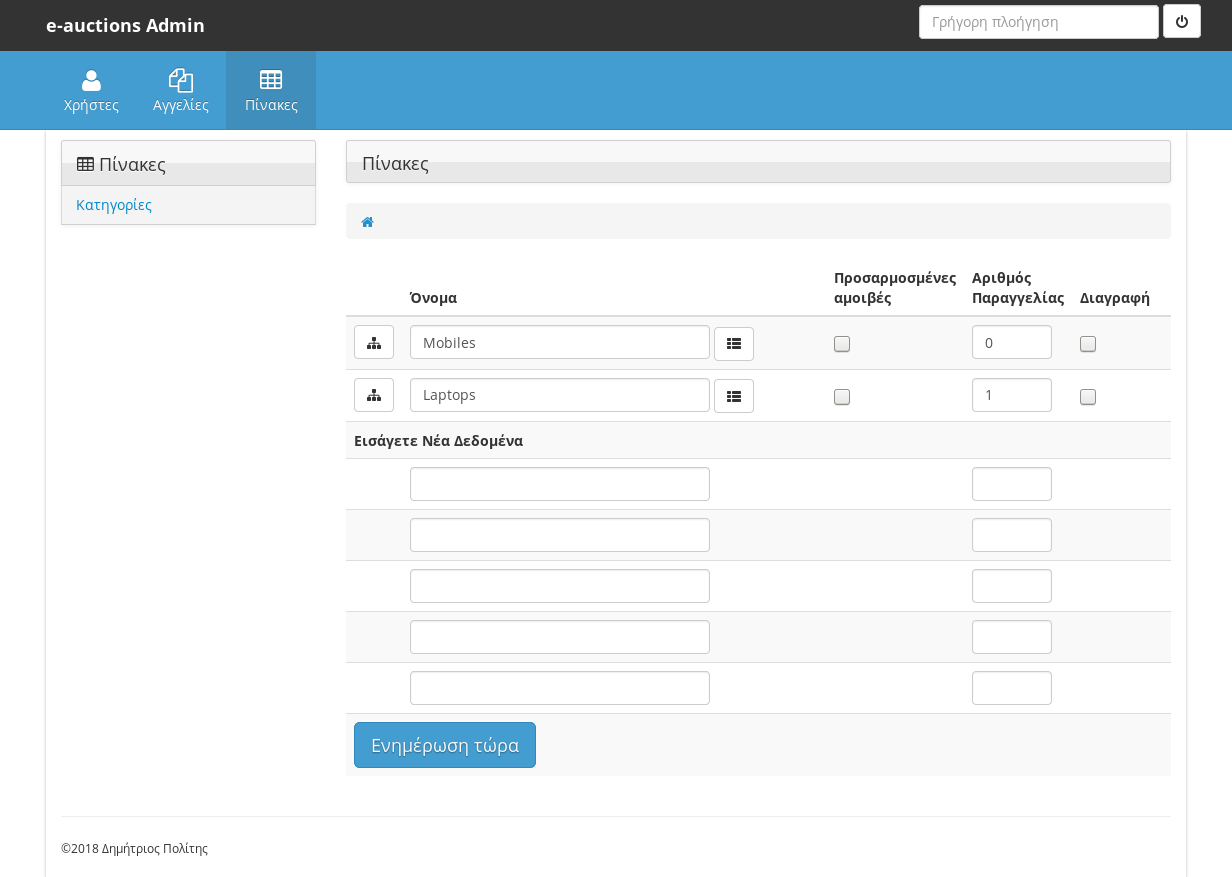
\includegraphics[width=0.8\textwidth, height=8cm]{Screenshot-2018-1-14-e-auctions-Admin-1}
\caption{Φόρμα Διαχείρησης Κατηγοριών Προϊόντων}
\label{fig:category_admin}
\end{figure}

\subsection{Λειτουργικότητα Δημοπρασιών}
Εάν ένας χρήστης με ιδιότητα πωλητή ή αγοραστή εισέλθει στο σύστημα με τα διαπιστευτήριά του, μπορεί αναλόγως το ρόλο που του έχει δοθεί στο \textlatin{admin panel}, να δημιουργήσει μια δημοπρασία ή να ποντάρει σε αυτή. Στην εικόνα~\ref{fig:auction_new} παρουσιάζεται μια από τις φόρμες του οδηγού καταχώρησης νέας δημοπρασίας από ένα πωλητή.
\begin{figure}[H]
\centering
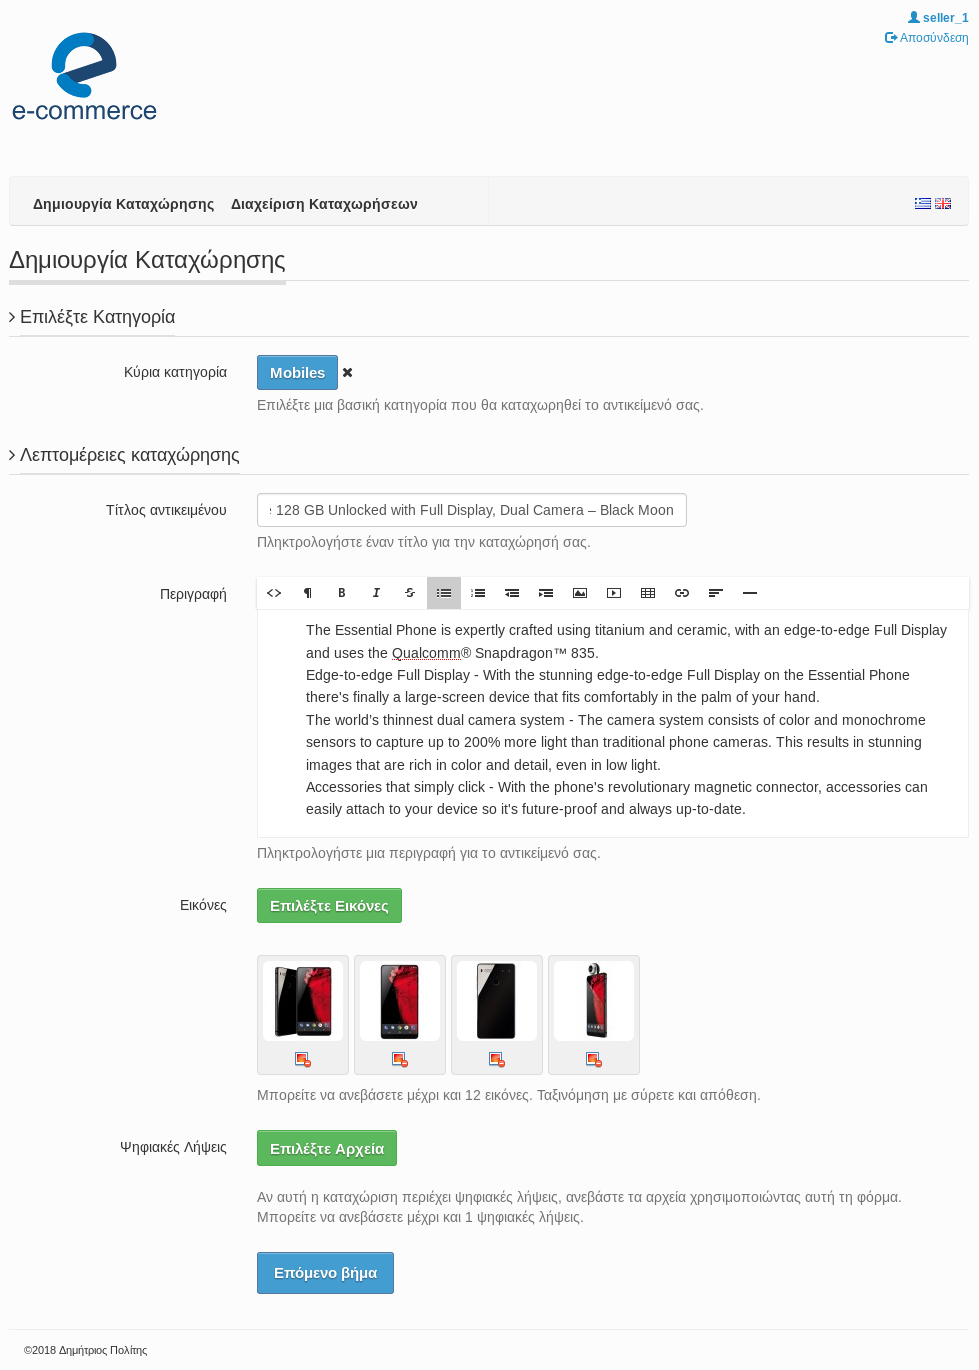
\includegraphics[width=0.8\textwidth, height=8cm]{Screenshot-2018-1-14-Sell-e-auctions}
\caption{Φόρμα Καταχώρησης Δημοπρασιών}
\label{fig:auction_new}
\end{figure}

Όταν ο χρήστης έχει το ρόλο αγοραστή (\textlatin{bidder}) ή παρατηρητή (\textlatin{spectator}) μπορεί να έχει πρόσβαση στις σελίδες προόδου της δημοπρασίας, αλλά μπορεί να αλληλεπιδρά με αυτές και να ποντάρει μόνο εφόσον έχει το ρόλο του πωλητή. Στην εικόνα~\ref{fig:auction_bid} παρουσιάζεται μια από τις φόρμες του οδηγού καταχώρησης νέου "χτυπηματος" (\textlatin{bidding} δημοπρασίας από έναν αγοραστή.
\begin{figure}[H]
\centering
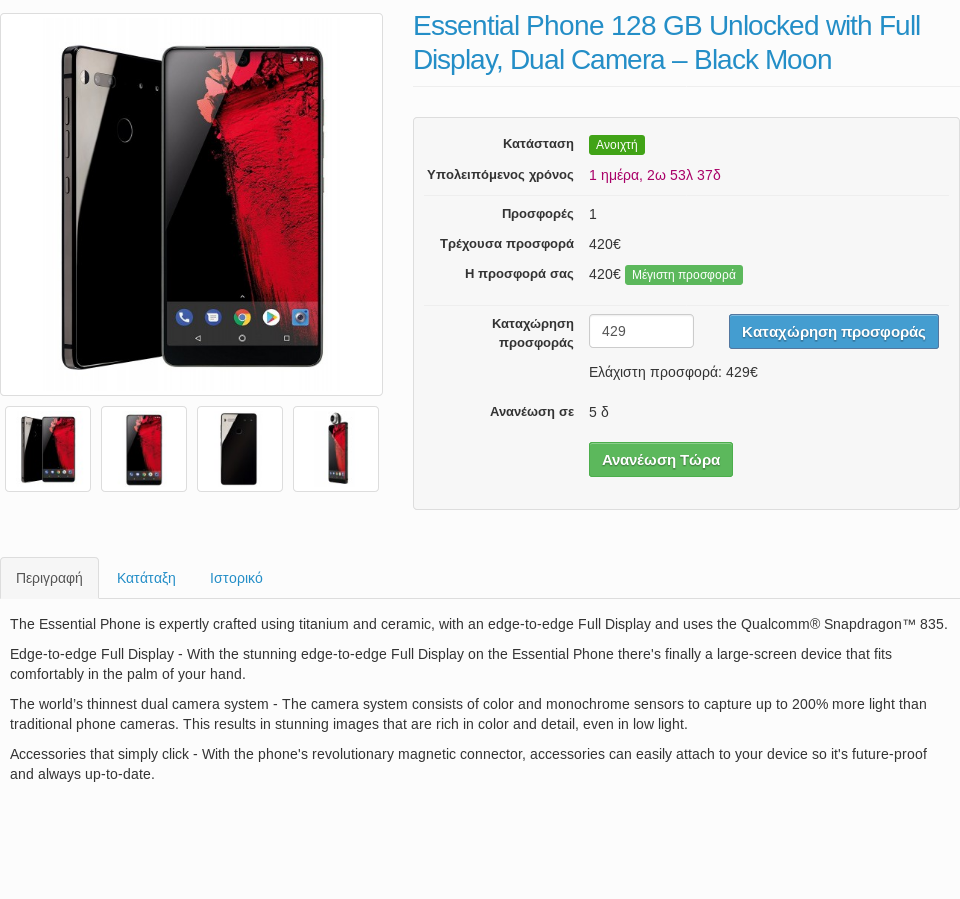
\includegraphics[width=0.8\textwidth, height=8cm]{Screenshot-2018-1-14-Essential-Phone-128-GB-Unlocked-with-Full-Display-Dual-Camera-Black-Moon-1}
\caption{Φόρμα Καταχώρησης Χτυπημάτων}
\label{fig:auction_bid}
\end{figure}

\section{Συμπεράσματα}
Στο παρόν, παρουσιάστηκε η διαδικασία ανάπτυξης καθώς και η λειτουργικότητα μιας ιστοσελίδας ηλεκτρονικών δημοπρασιών. Έγινε αναφορά σε βασικές έννοιες του ηλεκτρονικού εμπορίου και των ηλεκτρονικών δημοπρασιών. Στη συνέχεια περιγράφηκαν τα εργαλεία τα οποία χρησιμοποιήθηκαν για την ανάπτυξη του ιστοτόπου της εργασίας και ο τρόπος με τον οποίο αυτοματοποιήθηκαν και συνδυάστηκαν για την παραγωγή του τελικού αποτελέσματος, μετά και τη διαδικασία αποσφαλμάτωσης. Τέλος παρουσιάστηκαν οι βασικές λειτουργίες της σελίδας με συνοπτικό τρόπο και τη βοήθεια ανάλογων \textlatin{screenshots}.

Η ιστοσελίδα της εργασίας παρέχει πλήρη λειτουργικότητα διεξαγωγής των δημοπρασιών, με αυτόματη ανανέωση της σελίδας και ενημέρωση των χρηστών για την πορεία της διαδικασίας. Εκτός αυτού, με τη διάκριση των ρόλων των χρηστών και την ασφαλή αυθεντικοποίηση μέσω φορμών εισαγωγής στοιχείων, παρέχεται η απαιτούμενη διασφάλιση της διαδικασίας. Λειτουργικότητες που δεν ενσωματώθηκαν στην εργασία, όπως πληρωμές με τραπεζικές κάρτες, \textlatin{paypal} κ.α παραλήφθηκαν για λόγους κόστους, όπως αναλύθηκε στο~\ref{phpprobid}.

\begin{appendices}
\chapter{Αρχείο Ρύθμισης Εικονικής Μηχανής \textlatin{Vagrantfile}}\label{AppA}
\selectlanguage{english}
\inputminted[linenos, fontsize=\scriptsize, breaklines, baselinestretch=1]{ruby}{sources/Vagrantfile}
\selectlanguage{greek}
\end{appendices}

\appendix

\bibliographystyle{babplain}
\bibliography{e-commerce}

\end{document}